% Communication with make =============================================

\def\GRAPHPATH{localgraphics}

\ifdefined\HANDOUT
  \documentclass[handout,aspectratio=1610,dvipsnames]{beamer}
  \def\GRAPHPATH{graphics}
\else
  \documentclass[aspectratio=1610,dvipsnames]{beamer}
\fi

\ifdefined\TITLE
\else
  \def\TITLE{}
\fi

\usepackage[ngerman]{babel}
\usepackage{ifthen}
\usepackage{color}
\usepackage{colortbl}
\usepackage{textcomp}
\usepackage{multirow}
\usepackage{nicefrac}
\usepackage{multicol}
\usepackage{langsci-gb4e}
\usepackage{verbatim}
\usepackage{cancel}
\usepackage{graphicx}
\usepackage{hyperref}
\usepackage{verbatim}
\usepackage{boxedminipage}
\usepackage{adjustbox}
\usepackage{rotating}
\usepackage{booktabs}
\usepackage{bbding}
\usepackage{pifont}
\usepackage{multicol}
\usepackage{stmaryrd}
\usepackage{FiraSans}
\usepackage{soul}
\usepackage{tikz}
\usepackage[linguistics]{forest}
\usepackage[maxbibnames=99,
  maxcitenames=2,
  uniquelist=false,
  backend=biber,
  doi=false,
  url=false,
  isbn=false,
  bibstyle=biblatex-sp-unified,
  citestyle=sp-authoryear-comp]{biblatex}

% Biblatex ============================================================

\addbibresource{rs.bib}

% Colors ==============================================================

\definecolor{grau}{rgb}{0.5,0.5,0.5}
\definecolor{lg}{rgb}{0.8,0.8,0.8}
\definecolor{trueblue}{rgb}{0.3,0.3,1}
\definecolor{ltb}{rgb}{0.8,0.8,1}
\definecolor{lgr}{rgb}{0.5,1,0.5}
\definecolor{orongsch}{RGB}{255,165,0}
\definecolor{gruen}{rgb}{0,0.4,0}
\definecolor{rot}{rgb}{0.7,0.2,0.0}
\definecolor{tuerkis}{RGB}{63,136,143}
\definecolor{braun}{RGB}{108,71,65}
\definecolor{blaw}{rgb}{0,0,0.9}
\newcommand{\gruen}[1]{\textcolor{gruen}{#1}}
\newcommand{\blaw}[1]{\textcolor{blaw}{#1}}
\newcommand{\rot}[1]{\textcolor{rot}{#1}}
\newcommand{\blau}[1]{\textcolor{trueblue}{#1}}
\newcommand{\orongsch}[1]{\textcolor{orongsch}{#1}}
\newcommand{\grau}[1]{\textcolor{grau}{#1}}
\newcommand{\whyte}[1]{\textcolor{white}{#1}}
\newcommand{\tuerkis}[1]{\textcolor{tuerkis}{#1}}
\newcommand{\braun}[1]{\textcolor{braun}{#1}}

% Newcommands =========================================================

\newcommand{\Dim}{\cellcolor{lg}}
\newcommand{\Dimblue}{\cellcolor{ltb}}
\newcommand{\Dimgreen}{\cellcolor{lgr}}
\newcommand{\Sub}[1]{\ensuremath{_{\text{#1}}}}
\newcommand{\Up}[1]{\ensuremath{^{\text{#1}}}}
\newcommand{\UpSub}[2]{\ensuremath{^{\text{#1}}_{\text{#2}}}}
\newcommand{\Spur}[1]{t\Sub{#1}}
\newcommand{\Ti}{\Spur{1}}
\newcommand{\Tii}{\Spur{2}}
\newcommand{\Tiii}{\Spur{3}}
\newcommand{\Tiv}{\Spur{4}}
\newcommand{\Ck}{\CheckmarkBold}
\newcommand{\Fl}{\XSolidBrush}
\newcommand{\xxx}{\hspaceThis{[}}
\newcommand{\zB}{z.\,B.\ }
\newcommand{\down}[1]{\ensuremath{\mathrm{#1}}}
\newcommand{\Zeile}{\vspace{\baselineskip}}
\newcommand{\Halbzeile}{\vspace{0.5\baselineskip}}
\newcommand{\Viertelzeile}{\vspace{0.25\baselineskip}}
\newcommand{\KTArr}[1]{\ding{226}~\textit{#1}~\ding{226}}
\newcommand{\Ast}{*}
\newcommand{\SL}{\ensuremath{\llbracket}}
\newcommand{\SR}{\ensuremath{\rrbracket}}
\def\lspbottomrule{\bottomrule}
\def\lsptoprule{\toprule}
\newcommand{\Sw}[1]{\begin{sideways}#1\end{sideways}}
\newcommand{\Lab}{\ensuremath{\langle}}
\newcommand{\Rab}{\ensuremath{\rangle}}
\newcommand{\AbUmlautBreaker}{}
\ifdefined\HANDOUT
  \renewcommand{\AbUmlautBreaker}{\ /}
\fi
\newcommand{\LocStrutGrph}{\hspace{0.1\textwidth}}
\newcommand{\Nono}{---}

% Beamer ==============================================================

\usetheme[hideothersubsections]{PaloAlto}

\renewcommand<>{\rot}[1]{%
  \alt#2{\beameroriginal{\rot}{#1}}{#1}%
}
\renewcommand<>{\blau}[1]{%
  \alt#2{\beameroriginal{\blau}{#1}}{#1}%
}
\renewcommand<>{\orongsch}[1]{%
  \alt#2{\beameroriginal{\orongsch}{#1}}{#1}%
}
\renewcommand<>{\gruen}[1]{%
  \alt#2{\beameroriginal{\gruen}{#1}}{#1}%
}

\setbeamercolor{alerted text}{fg=trueblue}

\addtobeamertemplate{navigation symbols}{}{%
    \usebeamerfont{footline}%
    \usebeamercolor[fg]{footline}%
    \hspace{1em}%
    \insertframenumber/\inserttotalframenumber
}

\newcounter{lastpagemainpart}

\resetcounteronoverlays{exx}

\AtBeginSection[]{
  \begingroup
  \setbeamertemplate{navigation symbols}{}
  \begin{frame}[noframenumbering]
  \vfill
  \centering
  \begin{beamercolorbox}[sep=8pt,center,shadow=true,rounded=true]{title}
    \usebeamerfont{title}\insertsectionhead\par%
  \end{beamercolorbox}
  \vfill
  \end{frame}
  \endgroup
}

\setbeamertemplate{navigation symbols}{\insertframenumber/\inserttotalframenumber\hspace{5em}}

% Tikz ================================================================

\usetikzlibrary{positioning,arrows,cd}
\tikzset{>=latex}

% Forest

\forestset{
  Ephr/.style={draw, ellipse, thick, inner sep=2pt},
  Eobl/.style={draw, rounded corners, inner sep=5pt},
  Eopt/.style={draw, rounded corners, densely dashed, inner sep=5pt},
  Erec/.style={draw, rounded corners, double, inner sep=5pt},
  Eoptrec/.style={draw, rounded corners, densely dashed, double, inner sep=5pt},
  Ehd/.style={rounded corners, fill=gray, inner sep=5pt,
    delay={content=\whyte{##1}}
  },
  Emult/.style={for children={no edge}, for tree={l sep=0pt}},
  phrasenschema/.style={for tree={l sep=2em, s sep=2em}},
  decide/.style={draw, chamfered rectangle, inner sep=2pt},
  finall/.style={rounded corners, fill=gray, text=white},
  intrme/.style={draw, rounded corners},
  yes/.style={edge label={node[near end, above, sloped, font=\scriptsize]{Ja}}},
  no/.style={edge label={node[near end, above, sloped, font=\scriptsize]{Nein}}},
  sake/.style={tier=preterminal},
  ake/.style={
    tier=preterminal
    },
}

\tikzset{
    invisible/.style={opacity=0,text opacity=0},
    visible on/.style={alt=#1{}{invisible}},
    alt/.code args={<#1>#2#3}{%
      \alt<#1>{\pgfkeysalso{#2}}{\pgfkeysalso{#3}}
    },
}

\forestset{
  visible on/.style={
    for tree={
      /tikz/visible on={#1},
      edge+={/tikz/visible on={#1}}}}}

\useforestlibrary{edges}

\forestset{
  narroof/.style={roof, inner xsep=-0.25em, rounded corners},
  forky/.style={forked edge, fork sep-=7.5pt},
  bluetree/.style={for tree={trueblue}, for children={edge=trueblue}},
  orongschtree/.style={for tree={orongsch}, for children={edge=orongsch}},
  rottree/.style={for tree={rot}, for children={edge=rot}},
  gruentree/.style={for tree={gruen}, for children={edge=gruen}},
  tuerkistree/.style={for tree={tuerkis}, for children={edge=tuerkis}},
  brauntree/.style={for tree={braun}, for children={edge=braun}},
}


% Drawing sonority diagrams =========================================== 

\makeatletter

\long\def\ifnodedefined#1#2#3{%
  \@ifundefined{pgf@sh@ns@#1}{#3}{#2}}

\newcommand\aeundefinenode[1]{%
  \expandafter\ifx\csname pgf@sh@ns@#1\endcsname\relax
  \else
    \typeout{Undefining node "#1"}%
    \global\expandafter\let\csname pgf@sh@ns@#1\endcsname\relax
  \fi
}

\newcommand\aeundefinethesenodes[1]{%
  \foreach \myn  in {#1}
    {%
      \ifnodedefined{\myn}{%
      \expandafter\aeundefinenode\expandafter{\myn}%
    }{}
    }%
}

\newcommand\aeundefinenumericnodes{%
  \foreach \myn in {1,2,...,50}
    {%
      \ifnodedefined{\myn}{%
      \expandafter\aeundefinenode\expandafter{\myn}%
    }{}
    }%
}
\makeatother

\newcommand{\plo}{0}
\newcommand{\fri}{0.5}
\newcommand{\nas}{1}
\newcommand{\liq}{1.5}
\newcommand{\vok}{2}

% Save text.
\newcommand{\lastsaved}{}
\newcommand{\textsave}[1]{\gdef\lastsaved{#1}#1}

\newcommand{\SonDiag}[2][0]{%
  \begin{tikzpicture}
    \textsave{.}
    \tikzset{
      normalseg/.style={fill=white},
      extrasyll/.style={circle, draw, fill=white},
      sylljoint/.style={diamond, draw, fill=white}
    }
    \node at (0,\plo) {P};
    \node at (0,\fri) {F};
    \node at (0,\nas) {N};
    \node at (0,\liq) {L};
    \node at (0,\vok) {V};

    % Draw the helper lines if required.
    \ifthenelse{\equal{#1}{0}}{}{%
      \foreach \y in {\plo, \fri, \nas, \liq,\vok} {%
	\draw [dotted, |-|] (0.25, \y) -- (#1.75, \y);
      }
    }

    \foreach [count=\x from 1, remember=\x as \lastx] \p / \y / \g in #2 {
      \ifthenelse{\equal{\y}{-1}}{\textsave{.}}{%

	% Draw the node, either plain, as Silbenbgelenk, or as extrasyllabic.
        \ifthenelse{\equal{\g}{1}}{%
	  \node (\x) [sylljoint] at (\x, \y) {\p};
	}{%
	  \ifthenelse{\equal{\g}{2}}{%
	    \node (\x) [extrasyll] at (\x, \y) {\p};
	  }{%
	    \node (\x) [normalseg] at (\x, \y) {\p};
	  }
	}

	% Draw the connection unless the previous node was not or was empty.
	\ifthenelse{\NOT\equal{\lastsaved}{.}}{%
	  \draw [->] (\lastx) to (\x);
	}{}
	\textsave{1}
      }
    }
    \aeundefinenumericnodes
  \end{tikzpicture}
}


% Meta ================================================================

\title[Morphologie, Lexikon]{Einführung in die Morphologie und Lexikologie\\\TITLE}
\author{Roland Schäfer}
\institute{Institut für Germanistische Sprachwissenschaft\\Friedrich-Schiller-Universität Jena}
\date{Diese Version ist vom \today.\\\Zeile%
  \scriptsize \grau{stets aktuelle Fassungen: \url{https://github.com/rsling/SE-Einfuehrung-in-die-Morphologie-und-Lexikologie}}}

\begin{document}

\begingroup
\setbeamertemplate{navigation symbols}{}
\begin{frame}[noframenumbering]
 \titlepage
\end{frame}
\endgroup

\ifdefined\LECTURE
  \include{includes/\LECTURE}
\else

  \makeatletter
  \setbeamertemplate{section in sidebar}{\vspace{0.25\baselineskip}\vbox{%
      \beamer@sidebarformat{3pt}{section in sidebar}{\insertsectionhead}\vspace{-0.25\baselineskip}}}
  \setbeamertemplate{section in sidebar shaded}{\vspace{0.25\baselineskip}\vbox{%
      \beamer@sidebarformat{3pt}{section in sidebar shaded}{\insertsectionhead}\vspace{-0.25\baselineskip}}}
  \setbeamertemplate{subsection in sidebar}{\hspace{1em}\vbox{%
    \beamer@sidebarformat{3pt}{subsection in sidebar}{\insertsubsectionhead}\vspace{-0.5\baselineskip}}}
  \setbeamertemplate{subsection in sidebar shaded}{\hspace{1em}\vbox{%
      \beamer@sidebarformat{3pt}{subsection in sidebar shaded}{\insertsubsectionhead}\vspace{-0.5\baselineskip}}}
  \makeatother

%   \begin{frame}
%     {Stand der Überarbeitung}
%     \begin{center}
%       \Large Dieser Foliensatz ist erst bis\\
%       einschließlich \alert{Vorlesung 10}\\
%       für das Wintersemester 2019\slash 2020 überarbeitet.
%     \end{center}
%   \end{frame}

  \section[Sprache]{Sprache \& Sprache und Lehramt}
  \let\woopsi\section\let\section\subsection\let\subsection\subsubsection
  
\begin{frame}
  {Grammatik im Germanistik-BA | Mein Ansatz}
  \onslide<+->
  \onslide<+->
  \alert{\Large "`Sie müssen lernen, Grammatik zu machen."'}\\
  (Peter Eisenberg, Vorlesung an der FU Berlin 2014)\\
  \Zeile
  \onslide<+->
  \begin{itemize}[<+->]
    \item Es geht mir nicht um Theorievermittlung.
    \item Sie sollen ein Bild davon bekommen, was das Deutsche\\
      grammatisch gesehen so alles kann.
    \item Wir können Ihnen nicht ansatzweise alles Wissen über\\
      die Grammatik des Deutschen beibringen.\\
      Sie müssen vielmehr \alert{Analysekompetenz} erwerben.
    \item Jede Beschreibung setzt irgendeine Theorie voraus,\\
      aber \alert{wir reden hier über Sprache, nicht über Linguistik}.
    \item Die Theorie wird also so klein wie möglich gehalten.
  \end{itemize}
\end{frame}

\section{Organisation}

\begin{frame}
  {Roland Schäfer}
  \onslide<+->
  \begin{itemize}[<+->]
    \item seit WS 2022\slash 2023 Professur für Grammatik und Lexikon
    \item 2020--2022 Forschungsstelle an der HU Berlin
    \item 2018 habilitiert an der HU Berlin\\
      (Germanistische Linguistik und allgemeine Sprachwissenschaft)
    \item 2007--2022 Mitarbeiter an der FU Berlin
    \item 2008 promoviert an der Uni Göttingen (Englische Syntax)
    \item 2002--2007 Mitarbeiter in der Sprachwissenschaft in Göttingen
    \item Studium in Marburg (Sprachwissenschaft, Japanologie)
  \end{itemize}
  \Zeile
  \onslide<+->
  Bitte nennen Sie mich nicht Professor\ldots\ \onslide<+-> Wenn Sie es tun, dann bitte richtig:\\
  \url{https://rolandschaefer.net/regeln-fur-den-mailverkehr/}
\end{frame}

\begin{frame}
  {Forschung}
  \onslide<+->
  \onslide<+->
  Linguistik (des Deutschen)\\
  \Halbzeile
  \begin{itemize}[<+->]
    \item kognitiv fundierte Grammatik
    \item Morphosyntax und Graphematik
    \item grammatische Variation ("`Zweifelsfälle"')
    \item individuelle Variation
    \item Registervariation
    \item Epistemologie
  \end{itemize}
  \Zeile
  \onslide<+->
  Methoden\\
  \Halbzeile
  \begin{itemize}[<+->]
    \item Korpuserstellung und -analyse
    \item verhaltensbasierte Experimente
    \item Fragen der statistischen Inferenz
  \end{itemize}
\end{frame}

\begin{frame}
  {Sitzungsverlauf}
  \onslide<+->
  \begin{itemize}[<+->]
    \item vorbereitende Lektüre: \citet{Schaefer2018b}
    \item 10--20 Minuten Besprechung der Take-Home-Übungen
    \item 20--30 Minuten interaktiver Vortrag
    \item 40--60 Minuten 
  \end{itemize}
\end{frame}

\section{Das Lexikon}

\begin{frame}
  {Lexika}
  \onslide<+->
  \onslide<+->
  Was ist für Sie ein "`Lexikon"'?\\
  \Zeile
  \onslide<+->
  \onslide<+->
  \begin{itemize}[<+->]
    \item Buch \onslide<+-> \ldots Aber auch das enthält nur:
    \item \alert{Datenbank} (inkl.\ Datenstruktur)
    \item Ort der Kodierung \alert{egal}
  \end{itemize}
  \onslide<+->
  \Zeile
  \alert{Lexikon (Linguistik) | Alle Wörter einer Sprache} \onslide<+-> \alert{$\Rightarrow$ stark strukturiert}\\
  \onslide<+->
  \textit{rot}, \textit{rote}, \textit{rotes}, \textit{rötlicheres}, \textit{Rot}, \textit{Rötlichkeiten}
\end{frame}

\begin{frame}
  {Inhalt\slash Daten in Lexika}
  \onslide<+->
  Was gehört für Sie in ein Lexikon? Und warum?\\
  \Zeile
  \onslide<+->
  \onslide<+->
  \begin{itemize}[<+->]
    \item phonetische\slash phonologische Information (über Wörter \ldots)\\
      \Viertelzeile
      \textit{Klee} \alert{[kleː]}
    \item morphologische Information\\
      \Viertelzeile
      \textit{Klee} [kleː] \alert{N mask.\ st.}
    \item (morpho-)syntaktische Information\\
      \Viertelzeile
      \textit{rennen} [ʁɛnən] V st.\ (\textit{rannte, gerannt}) \alert{itr.}
      \Halbzeile
    \item beim mentalen Lexikon ähnlich
      \Halbzeile
    \item \alert{Bedeutung?} \ldots nicht unbedingt \citep{Elman2009}
    \item Evidenz für einfache Verknüpfungen zwischen \alert{Formlexikon} und \alert{Weltwissen}
  \end{itemize}
\end{frame}

\section{Struktur im Lexikon | Bedeutung?}

\begin{frame}
  {Was heißt hier Struktur?}
  \onslide<+->
  Welche \alert{lexikalisch-semantischen Beziehungen} gibt es zwischen Wörtern?\\
  \onslide<+->
  \onslide<+->
  \Halbzeile
  \begin{itemize}[<+->]
    \item z.\,B.\ im Fall Substantiv $\Leftrightarrow$ Substantiv
    \item Verb $\Leftrightarrow$ Verb
    \item Adjektiv $\Leftrightarrow$ Adjektiv
    \item Substantiv $\Leftrightarrow$ Verb
    \item und so weiter
  \end{itemize}
  \onslide<+->
  \Zeile
  Ach, übrigens, merken Sie was? \onslide<+-> \alert{Substantiv, Verb, Adjektiv, \ldots}
\end{frame}

\begin{frame}
  {Lexikalische Semantik und Ontologie}
  \onslide<+->
  Was ist eine Ontologie?\\
  \onslide<+->
  \Zeile
  \centering 
  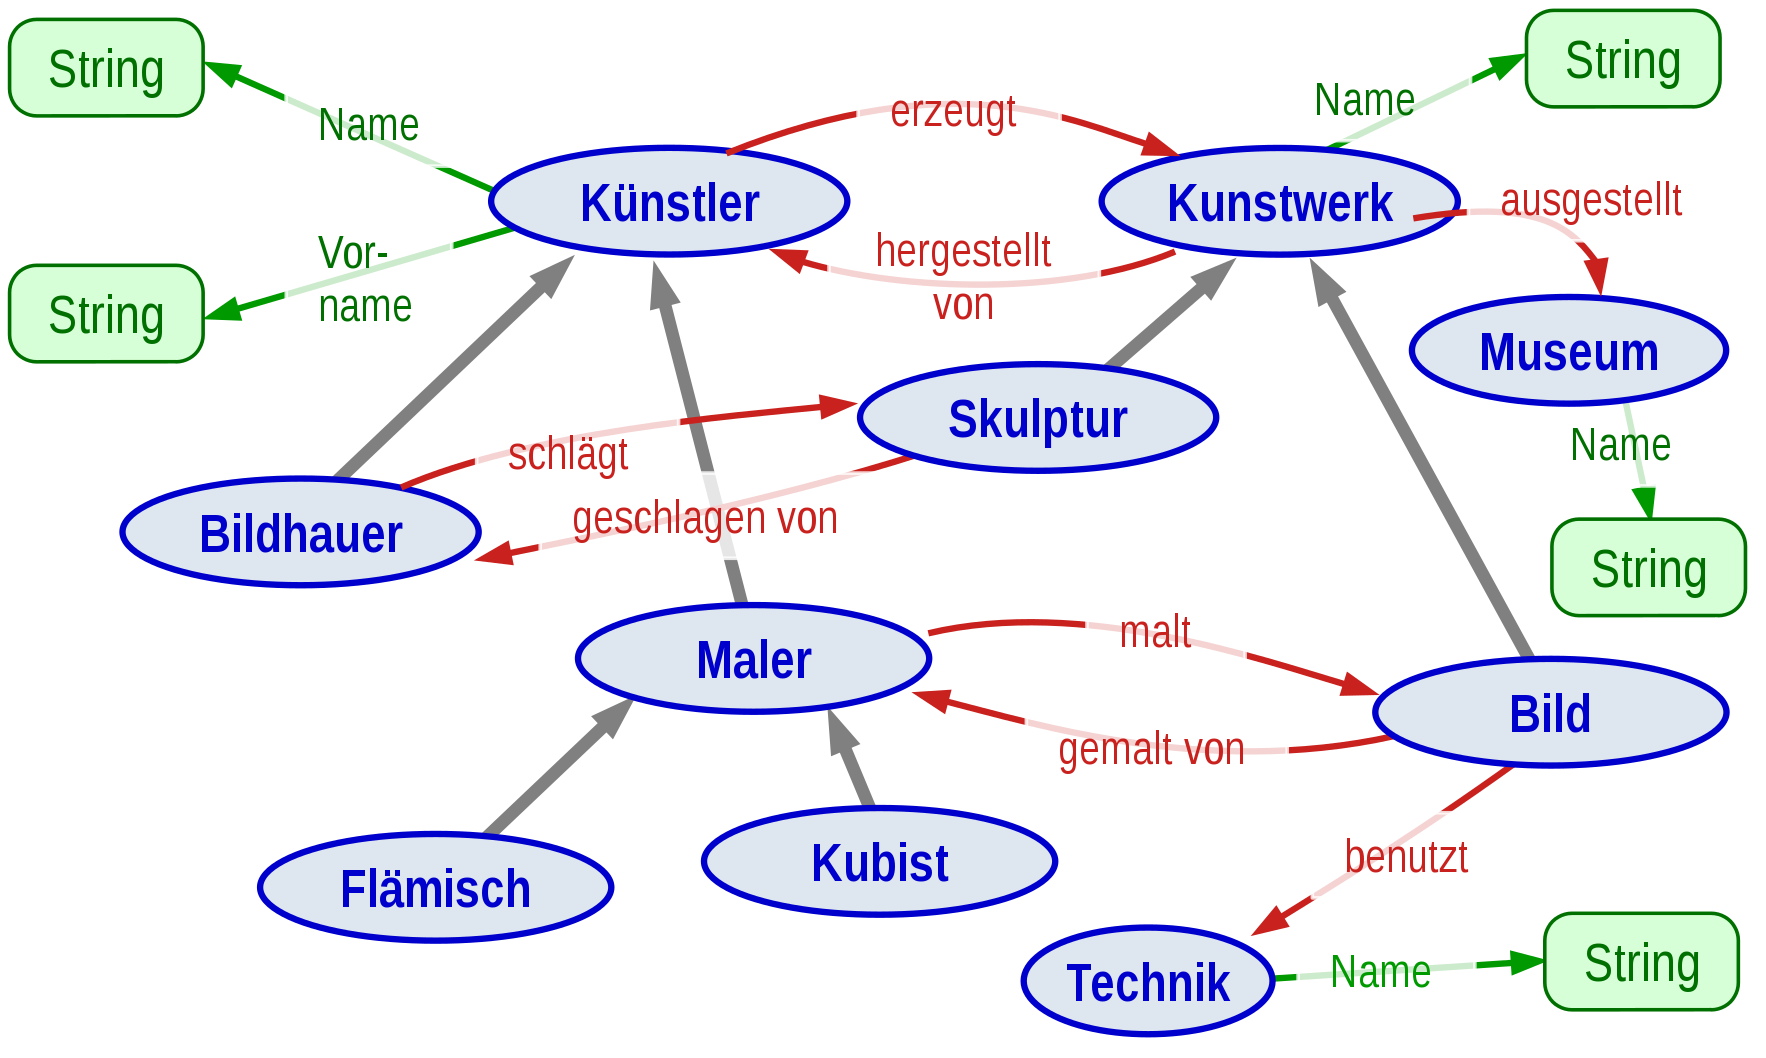
\includegraphics[height=0.7\textheight]{graphics/onto_typ}\\
  \Viertelzeile
  \grau{\tiny Quelle \url{https://de.wikipedia.org/wiki/Ontologie\_(Informatik)\#/media/Datei:Ontschichten.svg}}
\end{frame}

\begin{frame}
  {Ontologisch klassifizierte Objekte}
  \onslide<+->
  \onslide<+->
  \centering
  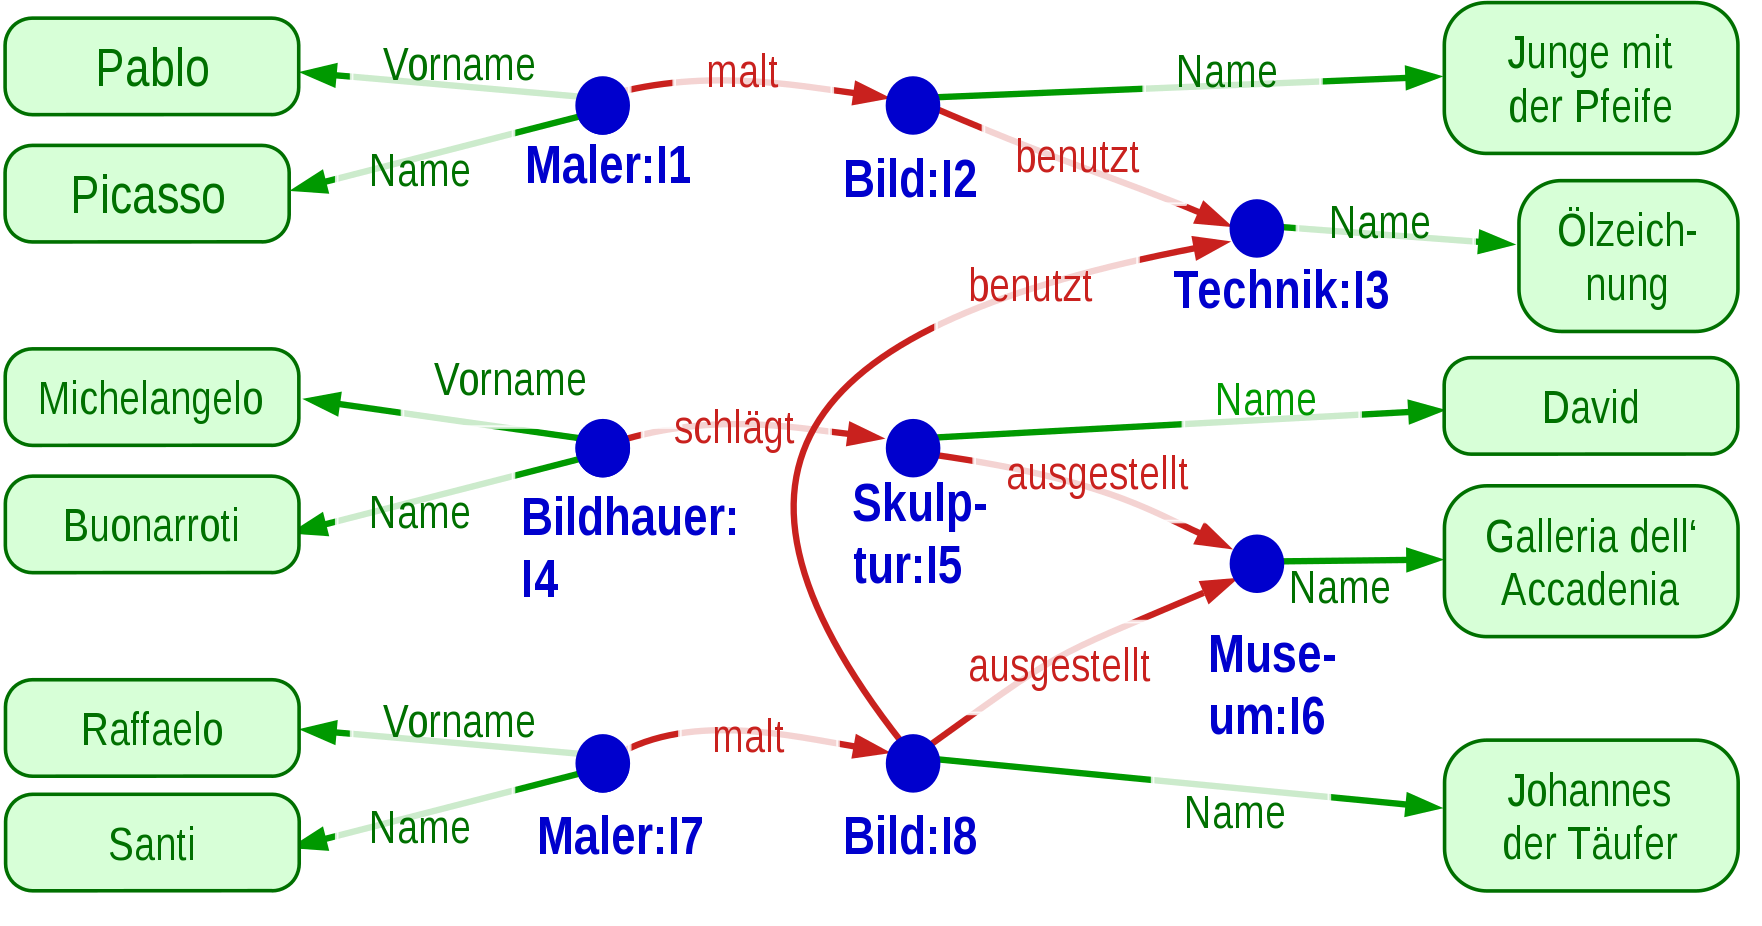
\includegraphics[height=0.7\textheight]{graphics/onto_tok}\\
  \Viertelzeile
  \grau{\tiny Quelle \url{https://de.wikipedia.org/wiki/Ontologie\_(Informatik)\#/media/Datei:Ontschichten.svg}}
\end{frame}

\section{Morphologie}

\begin{frame}
  {Wortklassen und Veränderlichkeit}
  \onslide<+->
  \onslide<+->
  Was für Wortklassen gibt es, und was unterscheidet sie \alert{grammatisch}?\\
  \onslide<+->
  \onslide<+->
  \Zeile
  \begin{itemize}[<+->]
    \item Veränderlichkeit (Flexion und Wortbildung)
    \item mögliche Arten der Veränderlichkeit
    \item syntaktische Kombinierbarkeit
  \end{itemize}
\end{frame}

\begin{frame}
  {Form und Funktion | Flexion}
  \onslide<+->
  \onslide<+->
  \begin{exe}
    \ex
    \begin{xlist}
      \ex \alert{Den Präsidenten} begrüßte \alert{der Dekan} äußerst respektlos.
       \onslide<+->
      \ex \alert{Der Dekan} begrüßte \alert{den Präsidenten} äußerst respektlos.
    \end{xlist}
    \onslide<+->
    \ex
    \begin{xlist}
      \ex \alert{Die Präsidentin} begrüßte \alert{die Dekanin} äußerst respektlos.
      \onslide<+->
      \ex \alert{Die Dekanin} begrüßte \alert{die Präsidentin} äußerst respektlos.
    \end{xlist}
  \end{exe}
  \onslide<+->
  \Zeile
  Formveränderungen lexikalischer Wörter \alert{schränken ihre möglichen grammatischen Funktionen und Relationen im Satz ein}\dots\\
  \onslide<+->
  \Halbzeile
  \dots und sie haben semantische und systemexterne Folgen.
\end{frame}

\begin{frame}
  {Unterklassen | Beispiel Substantive}
  \onslide<+->
  \onslide<+->
  Wie gliedert sich der substantivische Wortschatz weiter?
  \onslide<+->
  \onslide<+->
  \Zeile
  \begin{itemize}[<+->]
    \item \alert{Genus} | Maskulinum, Neutrum, Femininum
    \item Maskulinum | \alert{stark}, \alert{schwach}, \alert{gemischt} (oder so ähnlich)
    \item Femininum | Plural mit \textit{-e}, \textit{-en} oder endunglos (oder so ähnlich) 
  \end{itemize}
\end{frame}

\begin{frame}
  {Form und Funktion | Wortbildung}
  \onslide<+->
  \onslide<+->
  \begin{exe}
    \ex grün\alert{lich}, röt\alert{lich}, gelb\alert{lich}
    \onslide<+->
    \ex Neu\alert{igkeit}, Blöd\alert{heit}, Tauch\alert{er}, Heb\alert{ung}
    \onslide<+->
    \ex Fenster\alert{rahmen}, Tücher\alert{spender}, Glas\alert{korken}, Unter\alert{schrank}
  \end{exe}
  \onslide<+->
  \Zeile
  Formveränderungen von einem zu einem anderen lexikalischen Wort führen zu Bedeutungs- und kategorialen Veränderungen.
\end{frame}


\section{Struktur im Lexikon | Form}

\begin{frame}
  {Wortklassen | Morphosyntaktische Vorstrukturierung}
  \onslide<+->
  \onslide<+->
  \centering
  \resizebox{0.35\textwidth}{!}{
  \begin{minipage}{\textwidth}
  \centering
  \begin{forest}
    /tikz/every node/.append style={font=\footnotesize},
    for tree={l sep=2em, s sep=2.5em},
    [\textit{Wort}, intrme
      [{Hat\\Numerus?}, decide
        [\textit{flektierbar}, intrme, yes
          [{Ist finit\\flektierbar?}, decide
            [\textbf{Verb}, finall, yes]
            [\textit{Nomen}, intrme, no
              [{Hat festes\\Genus?}, decide
                [\textbf{Substantiv}, finall, yes]
                [{\textit{anderes}\\\textit{Nomen}}, intrme, no
                  [{Hat Stärke-\\flexion?}, decide
                    [\textbf{Adjektiv}, finall, yes]
                    [{\textit{Artikel\slash}\\\textit{Pronomen}}, intrme, no]
                  ]
                ]
              ]
            ]
          ]
        ]
        [\textit{nicht flektierbar}, intrme, no
        [{Hat Valenz-\slash\\Kasusrektion?}, decide
            [\textbf{Präposition}, finall, yes]
            [\textit{andere}, intrme, no
              [{Leitet Neben-\\Sätze ein?}, decide
                [\textbf{Komplementierer}, finall, yes]
                [{\textit{Partikel\slash}\\\textit{Adverb}}, intrme, no
                  [{Kann das Vor-\\feld besetzen?}, decide
                    [{\textit{Adverb\slash}\\\textit{Adkopula}}, intrme, yes
                      [{Wird typisch mit\\Kopula verwendet?}, decide
                        [\textbf{Adkopula}, finall, yes]
                        [\textbf{Adverb}, finall, no]
                      ]
                    ]
                    [\textit{Partikel}, intrme, no
                      [{Kann Sätze\\ersetzen?}, decide
                        [\textbf{Satzäquivalent}, finall, yes]
                        [\textit{andere}, intrme, no
                          [{Kann Konsti-\\tuenten verbinden?}, decide
                            [\textbf{Konjunktion}, finall, yes]
                            [\textit{Rest}, intrme, no]
                          ]
                        ]
                      ]
                    ]
                  ]
                ]
              ]
            ]
          ]
        ]
      ]
    ]
  \end{forest}
  \end{minipage}
  }
\end{frame}



\begin{frame}
  {Flexionsklassen der Substantive | Traditionell}
  \onslide<+->
  \onslide<+->
  \centering
  \resizebox{0.8\textwidth}{!}{
        \begin{tikzpicture}[every text node part/.style={align=center}]
      \node (MaskN)    at (2,4)   {\textbf{Maskulin}};
      \node (NeutN)    at (4,4)   {\textbf{Neutral}};
      \node (FemN)     at (8.5,4) {\textbf{Feminin}};

      \node (schwachN) at (0,2)   {\textbf{schwach}};
      \node (starkN)   at (2,2)   {\textbf{stark}};
      \node (gemistN)  at (4,2)   {\textbf{gemischt}};
      \node (sFlexN)   at (6.5,2) {\textbf{s-Flexion}};
      \node (s4N)      at (8.5,2) {\textbf{S4}};

      \node (EPlu)     at (0.5,0) {Plural\\\textit{\char`~e}};
      \node (ePlu)     at (2,0)   {Plural\\\textit{-e}};
      \node (erPlu)    at (3.5,0) {Plural\\\textit{\char`~er}};

      \node (enPlu)    at (7.5,0) {Plural\\\textit{-en}};
      \node (EnPlu)    at (9.5,0) {Plural\\\textit{\char`~e}};

      \draw (MaskN.south)  -- (schwachN.north);
      \draw (MaskN.south)  -- (starkN.north);
      \draw (MaskN.south)  -- (gemistN.north);
      \draw (MaskN.south)  -- (sFlexN.north);

      \draw (NeutN.south)  -- (starkN.north);
      \draw (NeutN.south)  -- (gemistN.north);
      \draw (NeutN.south)  -- (sFlexN.north);

      \draw (FemN.south)   -- (s4N.north);
      \draw (FemN.south)   -- (sFlexN.north);

      \draw [dashed] (starkN.south) -- (EPlu.north);
      \draw [dashed] (starkN.south) -- (ePlu.north);
      \draw [dashed] (starkN.south) -- (erPlu.north);

      \draw [dashed] (s4N.south)    -- (enPlu.north);
      \draw [dashed] (s4N.south)    -- (EnPlu.north);
    \end{tikzpicture}
  \begin{minipage}{\textwidth}
  \centering 
  \end{minipage}
  }
\end{frame}

\begin{frame}
  {Flexionsklassen der Substantive | Revidiert}
  \onslide<+->
  \onslide<+->
  \centering
  \resizebox{0.8\textwidth}{!}{
  \begin{minipage}{\textwidth}
  \centering 
    \begin{forest}
    [Substantive, calign=last, l sep+=2em
      [\textit{en}-Maskulina]
      [normale Flexion{,}\\differenziert\\nur nach\\Pluralbildung, l sep+=2em
        [\textit{\char`~er}\\nur Maskulina\\und Neutra\\(Kleinstklasse)]
        [\textit{\char`~e}\slash\textit{-e}\\Protoyp\\der \textbf{Maskulina}\\und \textbf{Neutra}]
        [\textit{-en}\\Prototyp\\der \textbf{Feminina}]
        [\textit{-s}\\lexikalisch oder\\phonotaktisch\\motiviert]
      ]
    ]
  \end{forest}
  \end{minipage}
  }
\end{frame}

\begin{frame}
  {Typenhierarchien}
  \onslide<+->
  \onslide<+->
  Vollständig formalisierte Grammatiktheorien wie HPSG \citep{Mueller2013a} \ldots\\
  \Zeile
  \onslide<+->
  \centering 
  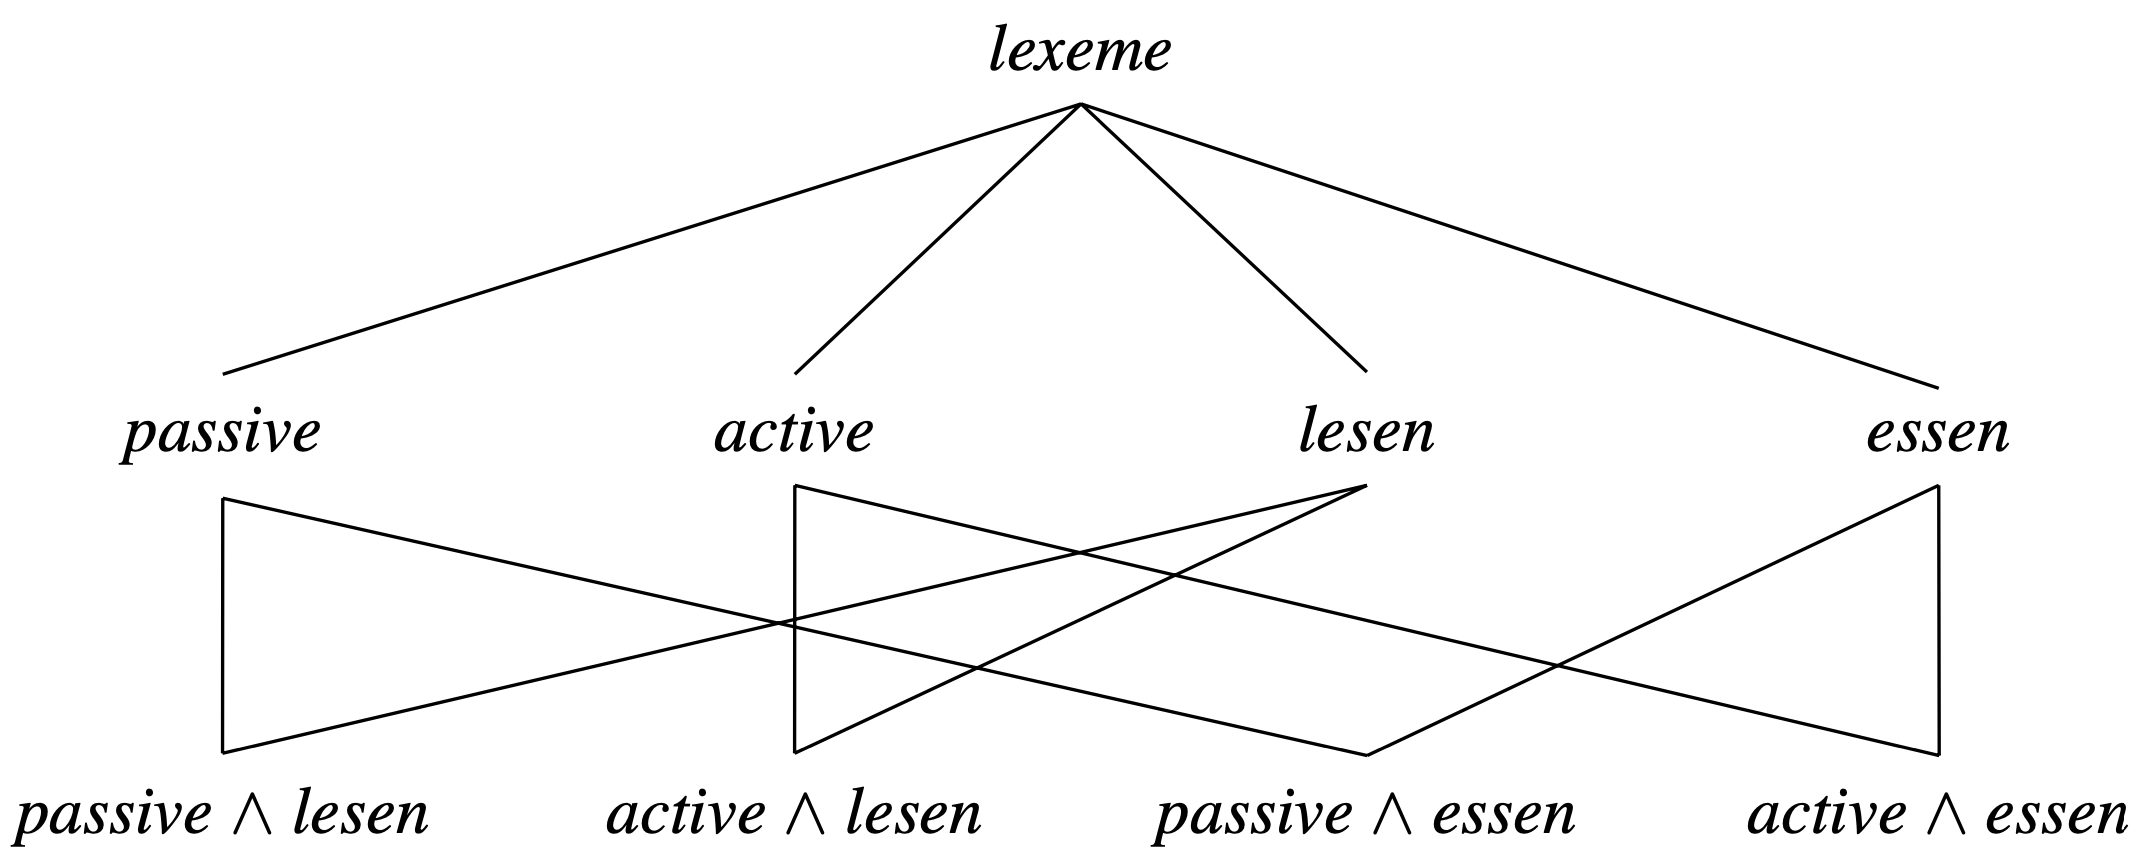
\includegraphics[width=0.8\textwidth]{graphics/typ_auto}\\
  \grau{\tiny Ausschnitt aus einer möglichen HPSG-Typenhierarchie. Die terminalen Typen müssen nicht händisch spezifiziert werden.}
\end{frame}

\begin{frame}
  {Wozu das Ganze?}
  \onslide<+->
  \onslide<+->
  Sprache ist nicht chaotisch, es gibt \alert{Regularitäten}, \\
  auch im \alert{Aufbau des Wortschatzes}.\\
  \Zeile
  \onslide<+->
  \alert{Gruppen von Einheiten} (hier: Wörtern) verhalten sich gleich oder ähnlich.\\
  \Zeile
  \onslide<+->
  Das \alert{hierarchisch gegliederte Lexikon} reflektiert diese Tatsache.\\
  \Zeile
  \onslide<+->
  Wäre Sprache chaotisch, wäre Sprache unbenutzbar und unlernbar.
\end{frame}

\begin{frame}
  {Semesterplan}
  Das Meiste dazu finden Sie in meiner Einführung \alert{EGBD3} \citep{Schaefer2018b}.\\
  \centering
  \Zeile
  \resizebox{0.7\textwidth}{!}{
  \begin{minipage}{\textwidth}
    \begin{enumerate}
      \item \grau{Morphologie und Lexikologie}
      \item Wörter und Wortstruktur
      \item Wortklassen
      \item Kern und Peripherie | Lehn- und Fremdwort
      \item Einführung Wortbildung | Komposition
      \item Derivation und Konversion
      \item Flexionsklassen der Nomina
      \item Flexionsklassen der Verben
      \item Relationen | Paradigma und Syntagma | Rektion
      \item Argumentstruktur und Valenz | Valenzklassen | Passiv | Statusrektion
      \item Unschärfe in Wortklassen und Wortbedeutung | Prototypen
      \item Sinnrelationen zwischen Lexemen
      \item Die Architektur des Wortschatzes
    \end{enumerate}
  \end{minipage}
}
\end{frame}

\begin{frame}
  {Nächste Woche}
  \onslide<+->
  \onslide<+->
  \alert{Wörter und Wortstruktur}\\
  \begin{itemize}[<+->]
    \item Lektüre EGBD3, Abschnitt 6.1
    \item Lektüre EGBD3, Kapitel 7
  \end{itemize}
\end{frame}

\begin{frame}
  {Interaktive Seminaraufgabe jetzt \ldots}
  \onslide<+->
  \Zeile
  \Zeile
  Suchen Sie im gegebenen Text (s.\ Handout)\\
  nach \alert{Wörtern mit identischen Worteigenschaften}.\\
  \Zeile
  Diese Formulierung ist absichtlich extrem weit gefasst!
\end{frame}


  \let\subsection\section\let\section\woopsi
  \section{Phonetik}
  \let\woopsi\section\let\section\subsection\let\subsection\subsubsection
  \section{Überblick}

\begin{frame}
  {Morphologie: Flexion und Wortbildung}
  \pause
  \begin{itemize}[<+->]
    \item \alert{Formveränderungen} und \alert{Merkmalsänderungen}
      \begin{itemize}[<+->]
        \item Veränderungen von Werten
        \item Veränderungen von Merkmalsaustattungen
      \end{itemize}
      \Halbzeile
    \item Morphe (= Wortbestandteile) und ihre Funktionen
    \item Morphe: alle Stämme und alle nicht-lexikalischen Morphe
      \Halbzeile
    \item statische und volatile Merkmale
    \item Wortbildung vs.\ Flexion, definiert anhand von Merkmalen
      \Zeile
    \item \citet[7.1]{Schaefer2018b}
  \end{itemize}
\end{frame}


\section{Stämme und Affixe}

\begin{frame}
  {Form und Funktion: Flexion}
  \pause
  \begin{exe}
    \ex
    \begin{xlist}
      \ex \alert{Den Präsidenten} begrüßte \alert{der Dekan} äußerst respektlos.
      \pause
      \ex \alert{Der Dekan} begrüßte \alert{den Präsidenten} äußerst respektlos.
    \end{xlist}
    \pause
    \ex
    \begin{xlist}
      \ex \alert{Die Präsidentin} begrüßte \alert{die Dekanin} äußerst respektlos.
      \pause
      \ex \alert{Die Dekanin} begrüßte \alert{die Präsidentin} äußerst respektlos.
    \end{xlist}
  \end{exe}
  \pause
  \Zeile
  Formveränderungen lexikalischer Wörter \alert{schränken ihre möglichen grammatischen Funktionen und Relationen im Satz ein}\dots\\
  \pause
  \Halbzeile
  \dots und sie haben semantische und systemexterne Folgen.

\end{frame}

\begin{frame}
  {Form und Funktion: Wortbildung}
  \pause
  \begin{exe}
    \ex grün\alert{lich}, röt\alert{lich}, gelb\alert{lich}
    \pause
    \ex Neu\alert{igkeit}, Blöd\alert{heit}, Tauch\alert{er}, Heb\alert{ung}
    \pause
    \ex Fenster\alert{rahmen}, Tücher\alert{spender}, Glas\alert{korken}, Unter\alert{schrank}
  \end{exe}
  \pause
  \Zeile
  Formveränderungen von einem zu einem anderen lexikalischen Wort führen zu Bedeutungs- und kategorialen Veränderungen.
\end{frame}

\begin{frame}
  {Markierungsfunktionen von Morphen I}
  \pause
  \begin{exe}
    \ex
    \begin{xlist}
      \ex{(der) \alert<4>{Berg}}
      \ex{(den) \alert<4>{Berg}}
      \ex{(dem) \alert<4>{Berg}}
      \ex{(des) \alert<5>{Berg}\rot<5>{-es}}
      \ex{(die) \alert<6>{Berg}\rot<6>{-e}}
      \ex{(der) \alert<6>{Berg}\rot<6>{-e}}
    \end{xlist}
    \pause
    \ex
    \begin{xlist}
      \ex{(der) \alert<8>{Mensch}}
      \ex{(den) \alert<9>{Mensch}\rot<9>{-en}}
      \ex{(dem) \alert<9>{Mensch}\rot<9>{-en}}
      \ex{(des) \alert<9>{Mensch}\rot<9>{-en}}
      \ex{(die) \alert<9>{Mensch}\rot<9>{-en}}
      \ex{(der) \alert<9>{Mensch}\rot<9>{-en}}
    \end{xlist}
  \end{exe}
\end{frame}

\begin{frame}
  {Markierungsfunktionen von Morphen II}
  \pause
  \begin{exe}
    \ex
    \begin{xlist}
      \ex{(ich) \alert<3>{kauf}\rot<3>{-e}}
      \ex{(du) \alert<4>{kauf}\rot<4>{-st}}
      \ex{(wir) \alert<5>{kauf}\rot<5>{-en}}
      \ex{(sie) \alert<5>{kauf}\rot<5>{-en}}
    \end{xlist}
  \end{exe}
\end{frame}

\begin{frame}
  {Morphe und Markierungsfunktionen}
  \pause
  \begin{itemize}[<+->]
    \item Formveränderungen:
      \begin{itemize}[<+->]
        \item oft nicht \alert{eine} Funktion
        \item \rot{Einschränkung} der möglichen Funktionen
      \end{itemize}
   \Halbzeile 
    \item \alert{Markierungsfunktion}: eine \alert{Reduktion}\\
      der möglichen Merkmale oder Werte einer Wortform
    \item zum Beispiel \textit{-en} bei schw.\ Maskulina: \rot{nicht} Nominativ Singular
    \item oder \textit{-en} bei Verben im Präsens: Plural und nicht adressatbezogen
      \Halbzeile
    \item \alert{Morphe = alle segmentalen Einheiten mit Markierungsfunktion}
    \item konkret: \alert{Stämme} und \alert{Affixe}
  \end{itemize}
\end{frame}

\begin{frame}
  {Stämme I}
  \pause
  \begin{exe}
    \ex
    \begin{xlist}
      \ex{(ich) \alert<5->{kauf}-e\\
        (du) \alert<5->{kauf}-st\\
        (ihr) \alert<5->{kauf}-t }
        \pause
        \ex{(ich) \alert<6->{kauf}-te\\
        (du) \alert<6->{kauf}-test\\
        (ihr) \alert<6->{kauf}-tet}
        \pause
        \ex{(ich habe) ge-\alert<7->{kauf}-t\\
        (du hast) ge-\alert<7->{kauf}-t\\
        (ihr habt) ge-\alert<7->{kauf}-t}
    \end{xlist}
  \end{exe}
\end{frame}

\begin{frame}
  {Stämme II}
  \begin{exe}
    \ex
    \begin{xlist}
      \ex{(ich) \alert<4->{nehm}-e\\
        (du) \rot<5->{nimm}-st\\
          (es) \rot<5->{nimm}-t\\
          (ihr) \alert<4->{nehm}-t}
        \pause
        \ex{(ich) \orongsch<6->{nahm}\\
        (du) \orongsch<6->{nahm}-st\\
          (ihr) \orongsch<6->{nahm}-t}
        \pause
        \ex{(ich habe) ge-\gruen<7->{nomm}-en\\
        (du hast) ge-\gruen<7->{nomm}-en\\
        (ihr habt) ge-\gruen<7->{nomm}-en}
    \end{xlist}
  \end{exe}
  \pause
  \pause
  \pause
  \pause
  \pause
  Der \alert{Stamm} kann nicht "`der unveränderliche Wortbestandteil"'\\
  eines lexikalischen Wortes (in einem Paradigma) sein.\\
  \Zeile
  \pause
  \alert{\dots aber der mit der Bedeutung, also der lexikalischen Markierungsfunktion}!
\end{frame}

\begin{frame}
  {Affixe}
  \pause
  \begin{exe}
    \ex
    \begin{xlist}
      \ex (ich) nehm\alert<6->{-e}
      \pause
      \ex (des) Berg\alert<7->{-es}
      \pause
      \ex Schön\alert<8->{-heit}
      \pause
      \ex \alert<9->{Un-}ding
    \end{xlist}
  \end{exe}
  \Zeile
  \pause
  \pause
  \pause
  \pause
  \pause
  \begin{itemize}[<+->]
    \item \alert{keine lexikalische Markierungsfunktion} (= keine eigene Bedeutung)
    \item \alert{nicht wortfähig} = nicht ohne Stamm verwendbar
  \end{itemize}
\end{frame}



\section{Merkmale in Flexion und Wortbildung}

\begin{frame}
  {Statische und volatile Merkmale}
  \pause
  \begin{itemize}[<+->]
    \item Eigenschaften: "`Rotsein"' (Erdbeere), "`325m hoch"' (Eiffelturm) usw.
    \item Merkmale: \alert{\textsc{Farbe}}, \alert{\textsc{Länge}} usw.
    \item Werte:
      \begin{itemize}[<+->]
        \item \alert{\textsc{Farbe}}: \rot{\textit{rot}}, \rot{\textit{grau}}, \ldots
        \item \alert{\textsc{Länge}}: \rot{\textit{3cm}}, \rot{\textit{325m}}, \ldots
      \end{itemize}
  \end{itemize}
  \pause
  \Halbzeile 
  \begin{exe}
    \ex
    \begin{xlist}
      \ex{Haus = [\textsc{Bed}: \gruen<12->{\textbf{\textit{haus}}}, \textsc{Klasse}: \gruen<12->{\textbf{\textit{subst}}}, \textsc{Gen}: \gruen<12->{\textbf{\textit{neut}}}, \textsc{Kas}: \orongsch<13->{\textit{nom}}, \textsc{Num}: \orongsch<13->{\textit{sg}}]}
      \pause
      \ex{Haus-es = [\textsc{Bed}: \gruen<12->{\textbf{\textit{haus}}}, \textsc{Klasse}: \gruen<12->{\textbf{\textit{subst}}}, \textsc{Gen}: \gruen<12->{\textbf{\textit{neut}}}, \textsc{Kas}: \orongsch<13->{\textit{gen}}, \textsc{Num}: \orongsch<13->{\textit{sg}}]}
      \pause
      \ex{Häus-er = [\textsc{Bed}: \gruen<12->{\textbf{\textit{haus}}}, \textsc{Klasse}: \gruen<12->{\textbf{\textit{subst}}}, \textsc{Gen}: \gruen<12->{\textbf{\textit{neut}}}, \textsc{Kas}: \orongsch<13->{\textit{nom}}, \textsc{Num}: \orongsch<13->{\textit{pl}}]}
    \end{xlist}
  \end{exe}
  \Halbzeile
  \pause
  \begin{itemize}[<+->]
    \item bei einem lexikalischen Wort:
      \begin{itemize}
        \item \gruen{statische Merkmale} wertestabil
        \item \orongsch{volatile Merkmale} werteverändernd im Paradigma
      \end{itemize}
  \end{itemize}
\end{frame}

\begin{frame}
  {Wortbildung in Abgrenzung zur Flexion}
  \pause
  \begin{exe}
    \ex
    \begin{xlist}
      \ex trocken (Adj) → \alert{Trocken}\rot{-heit} (Subst)
      \ex Kauf (Subst), Rausch (Subst) → \alert{Kauf}\rot{-rausch} (Subst)
      \ex gehen (V) → \alert{be}\rot{-gehen} (V)
    \end{xlist}
    \pause
    \ex
    \begin{xlist}
      \ex \alert{lauf}\rot{-en} (1\slash 3 Pl Prs Ind) → \alert{lauf}\rot{-e} (1 Sg Prs Ind)
      \ex \alert{Münze} (Sg) → \alert{Münze}\rot{-n} (Pl)
    \end{xlist}
  \end{exe}
  \pause
  \Halbzeile
  \begin{itemize}[<+->]
    \item Wortbildung
      \begin{itemize}[<+->]
        \item statische Merkmale geändert (Wortklasse, Bedeutung)
        \item \ldots oder gelöscht (alles außer Bedeutung: Erstglied bei Komposition)
        \item \ldots oder umgebaut (Valenz von Verben beim Applikativ)
        \item \alert{produktives Erschaffen neuer lexikalischer Wörter}
      \end{itemize}
  \Halbzeile
    \item Flexion
      \begin{itemize}
        \item Änderung der Werte volatiler Merkmale
        \item typisch: Anpassung an syntaktischen Kontext
      \end{itemize}
  \end{itemize}
\end{frame}

\section{Übung}

\begin{frame}
  {Stämme und Affixe}
  \Zeile
  \centering 
  Suchen Sie im Text der letzten Woche nach \alert{einfachen Wörtern}\\
  sowie \alert{Wörtern mit Stamm und Affix(en)}.\\
  \Zeile
  Versuchen Sie, die \alert{Markierungsfunktionen}\\
  der Stämme und Affixe zu bestimmen.
\end{frame}

\section{Vorschau}

\begin{frame}
  {Nächste Woche | Wortklassen}
  \Zeile
  \centering 
  Bitte lesen Sie \orongsch{unbedingt} \alert{Kapitel 6 (Wortklassen)} aus EGBD3!
\end{frame}

  
\fi

\makeatletter
\setcounter{lastpagemainpart}{\the\c@framenumber}
\makeatother

\appendix

\begin{frame}[allowframebreaks]
  {Literatur}
  \renewcommand*{\bibfont}{\footnotesize}
  \setbeamertemplate{bibliography item}{}
  \printbibliography
\end{frame}

\begin{frame}
  {Autor}
  \begin{block}{Kontakt}
    Prof.\ Dr.\ Roland Schäfer\\
    Institut für Germanistische Sprachwissenschaft\\
    Friedrich-Schiller-Universität Jena\\
    Fürstengraben 30\\
    07743 Jena\\[\baselineskip]
    \url{https://rolandschaefer.net}\\
    \texttt{roland.schaefer@uni-jena.de}
  \end{block}
\end{frame}

\begin{frame}
  {Lizenz}
  \begin{block}{Creative Commons BY-SA-3.0-DE}
    Dieses Werk ist unter einer Creative Commons Lizenz vom Typ \textit{Namensnennung - Weitergabe unter gleichen Bedingungen 3.0 Deutschland} zugänglich.
    Um eine Kopie dieser Lizenz einzusehen, konsultieren Sie \url{http://creativecommons.org/licenses/by-sa/3.0/de/} oder wenden Sie sich brieflich an Creative Commons, Postfach 1866, Mountain View, California, 94042, USA.
  \end{block}
\end{frame}

\mode<beamer>{\setcounter{framenumber}{\thelastpagemainpart}}

\end{document}
